\documentclass[12pt]{article}
\usepackage{graphicx}
\usepackage{geometry}
\usepackage{hyperref}
\usepackage{tabularx}
\usepackage{float}
\usepackage{setspace} % Add this package for line spacing

\geometry{a4paper, margin=1in}

\title{DRAM Timing Parameters}

\renewenvironment{abstract}
 {\par\noindent\textbf{\abstractname.}\ \ignorespaces}
 {\par\medskip}

\date{} % This removes the date

\begin{document}

% Set line spacing for the entire document
\setstretch{1.2} % Adjust to your preference (1.2 for slightly increased spacing)

% Custom title page content
\begin{titlepage}
    \centering
    {\Large \textbf{Assignment \# 1}} % Title in large bold text
    \vspace{0.2in}
		
		\vspace*{1in}
    
\includegraphics[width=0.3\textwidth]{./images/UetLogo.png} % Optional: add logo image
    \vspace{1in}
    
    {\large \textbf{Fall 2024}  \\ 
						\textbf{CSE-420 Embedded Systems}
						} % Author info
    \vspace{0.5in} 
    
    {\large \textbf{Name:} Ali Asghar \\ 
						\textbf{Registration:} 21PWCSE2059 \\
						\textbf{Section:} A \\
		} % Author info
    \vspace{0.5in}
		
    {\large Submitted to:\\ 
						\textbf{Dr.Asif Ali Khan} \\						
		} % Author info
    \vspace{0.5in}

    {\large Date:\\ 
						\textbf{7th November, 2024} \\						
		} % Author info
    \vspace{0.5in}
		
		{\large \textbf{Department of Computer Systems Engineering}\\ 
						\textbf{University of Engineering and Technology, Peshawar} \\						
		} % Author info
    \vspace{0.5in}
		
    \vfill
\end{titlepage}

% Start the main document without a duplicate title page
\newpage % Page break after cover page

%\section{Working of DRAM}
%Memory is organized into a grid-like pattern, with “rows” and “columns.” The data stored comes in blocks and is defined by the coordinates of the row and column. The steps for the memory controller to access data in SDRAM follow in order:

%First, the SDRAM is either in idle state or executing the previous operation. The controller issues the “active” command. It activates a certain row, as indicated by the address lines, in the SDRAM chip for accessing. This command typically takes a few clock cycles. After the delay, column address and either “read” or “write” command is issued. Typically the read or write command can be repeated every clock cycle for different column addresses (or a burst mode read can be performed). However, the read data isn't available until a few clock cycles later, because the memory is pipelined. When an access is requested to another row, the current row has to be deactivated by issuing the “precharge” command. The precharge command takes a few clock cycles before a new “active” command can be issued.

\section{Timing Parameters}
The timing parameters of DRAM (Dynamic Random Access Memory) are essential characteristics that define the latency and data transfer performance of DRAM modules. DRAM timing dictates how quickly memory cells can be accessed and refreshed and how fast data can be transferred to the processor. These parameters are especially crucial in DDR (Double Data Rate) DRAM technologies, where timing impacts the overall system performance. These timing parameters are measured in clock cycles and can be seen in figure \ref{fig:RAMTiming} below.


\begin{figure}[H]
	\centering
		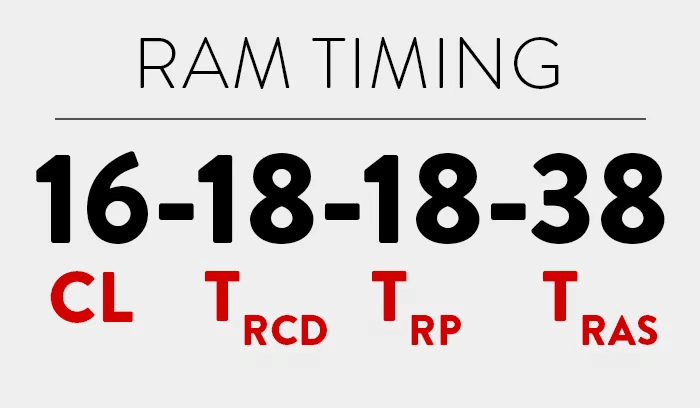
\includegraphics[width=0.5\textwidth]{./images/RAMTiming.png}
	\caption{RAM Timing on a DRAM Stick }
	\label{fig:RAMTiming}
\end{figure}

\subsection{CAS Latency (CL)}
CAS Latency (Column Access Strobe Latency), also known as “Access Time,” is the most important memory parameter and is the first of the series of numbers. It is the delay time between the moment a memory controller tells the memory module to access a particular memory column on a RAM memory module, and the moment the data from given array location is available on the module's output pins. In DDR SDRAM it is specified in clock cycles, while in asynchronous DRAM it is specified in nanoseconds\cite{website}.

The CAS latency is the delay, in clock cycles, between the registration of a READ command and the availability of the first piece of output data. The latency can be set to 1, 2 or 3 clocks. If a READ command is registered at clock edge n, and the latency is m clocks, the data will be available by clock edge n+m as shown in figure [\ref{fig:CAS_Latency1},\ref{fig:CAS_Latency2},\ref{fig:CAS_Latency3}]

\begin{figure}[H]
	\centering
		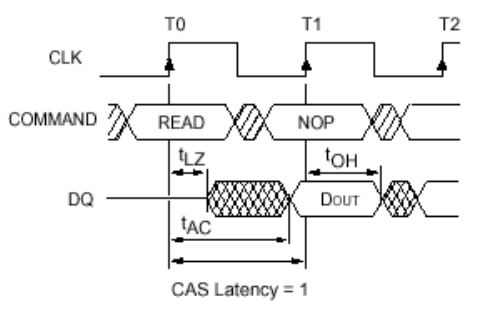
\includegraphics[width=0.5\textwidth]{./images/CAS_Latency1.png}
	\caption{CAS Latency = 1}
	\label{fig:CAS_Latency1}
\end{figure}

\begin{figure}[H]
	\centering
		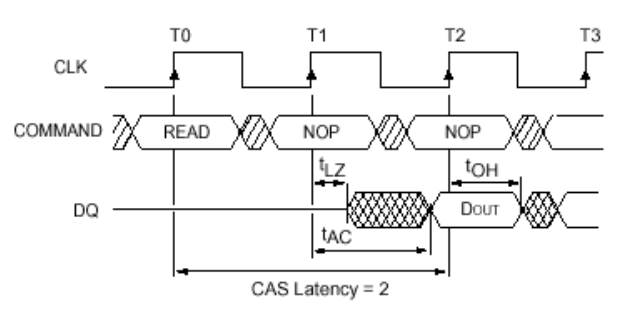
\includegraphics[width=0.75\textwidth]{./images/CAS_Latency2.png}
	\caption{CAS Latency = 2}
	\label{fig:CAS_Latency2}
\end{figure}

\begin{figure}[H]
	\centering
		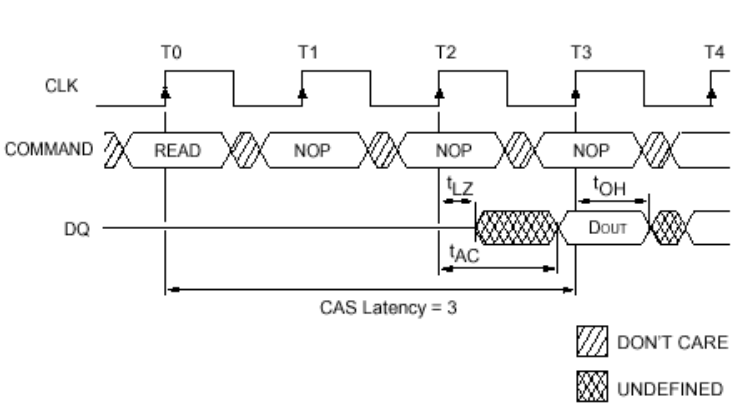
\includegraphics[width=1\textwidth]{./images/CAS_Latency3.png}
	\caption{CAS Latency = 3}
	\label{fig:CAS_Latency3}
\end{figure}

\subsection{RAS to CAS Delay (tRCD)}
tRCD stands for row address to column address delay time. Inside the memory, the process of accessing the stored data is accomplished by first activating the row then the column where it is located. tRCD is the time required between the memory controller asserting a row address strobe (RAS), and then asserting a column address strobe (CAS) during the subsequent read or write command. The lesser this time, the better it is, as the data will be read sooner.

\begin{figure}[H]
	\centering
		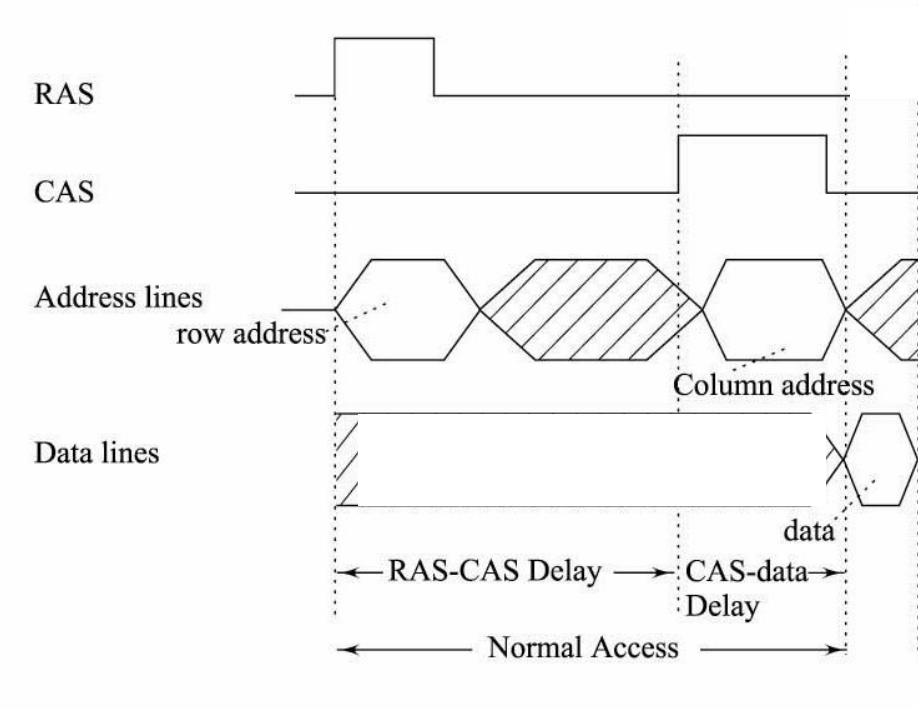
\includegraphics[width=0.5\textwidth]{./images/tRCD.png}
	\caption{tRCD shown as RAS to CAS delay}
	\label{fig:tRCD}
\end{figure}

\subsection{RAS Precharge (tRP)}
Whenever a new row is to be activated for the purpose of accessing a data bit, a command called “Precharge” needs to be issued to close the already activated row. RAS Precharge time, tRP is the number of clock cycles needed to terminate access to an open row of memory, and open access to the next row.
In simple words, tRP, specifies the time required to complete one row access, deactivate that row, reactivate the next row, and begin the next row access.
A simple graphical explanation of RAS Precharge (tRP) can be seen in figure \ref{fig:tRP}.

\begin{figure}[H]
	\centering
		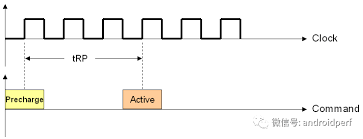
\includegraphics[width=0.75\textwidth]{./images/tRP.png}
	\caption{tRP delay \cite{cloudtencent}}
	\label{fig:tRP}
\end{figure}

\subsection{Active to Precharge Delay (tRAS)}
After an “Active” command is issued, another “Precharge” command cannot be issued until tRAS has elapsed. So, tRAS is the minimum number of clock cycles needed to access a certain row of data in the memory between the data request (Active) and the Precharge command. Basically, this parameter limits when the memory can start reading (or writing) a different row.

\begin{figure}[H]
	\centering
		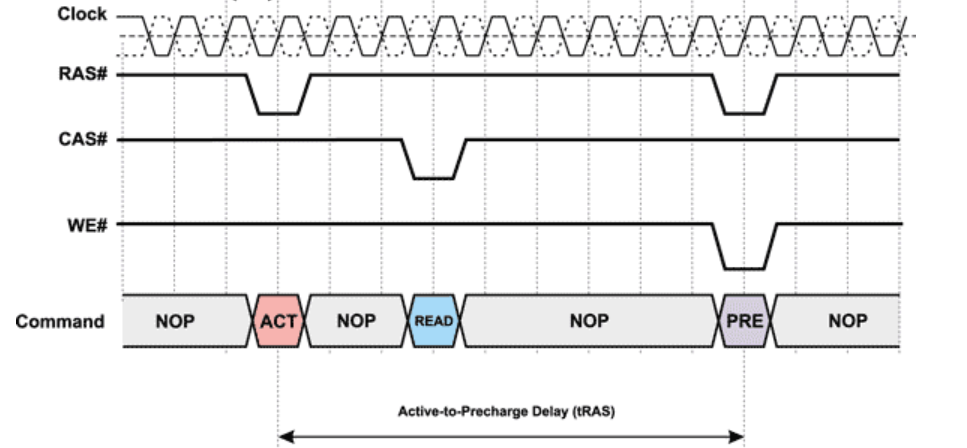
\includegraphics[width=0.75\textwidth]{./images/tRAS.png}
	\caption{tRAS delay \cite{tRASWeb}}
	\label{fig:tRAS}
\end{figure}



\bibliographystyle{IEEEtran} % or any other style you prefer
\bibliography{references}    % references.bib is the name of the .bib file
\end{document}
